\newpage
\subsection{Normale/Paralelle Lineare Funktionen}

Die zu einer Geraden normale Gerade erhält man durch den negativen Kehrwert: $K\bot = -\frac{1}{k}$

\hfill \break
Example normale Funktionenen:\\
\fboxrule=0.8pt \fcolorbox{black}{lightgray}{%
    \begin{tabular}[t]{@{}l@{}}
        $\textcolor{red}{y=\frac{3}{4}x}$      \\
        $\textcolor{green}{y_n=-\frac{4}{3}x}$ \\
    \end{tabular}}

\hfill \break
Example paralelle Funktionenen:\\
\fboxrule=0.8pt \fcolorbox{black}{lightgray}{%
    \begin{tabular}[t]{@{}l@{}}
        $\textcolor{blue}{y = 3x-1}$   \\
        $\textcolor{violet}{y = 3x+3}$ \\
    \end{tabular}}

\hfill \break
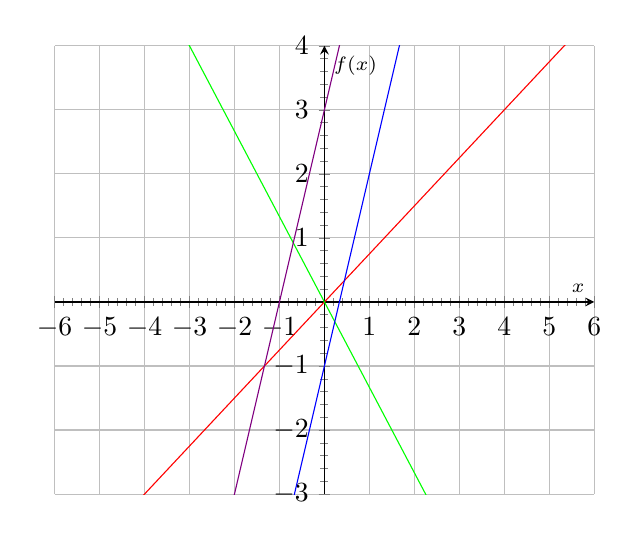
\begin{tikzpicture}[scale=1.0]
    \begin{axis}%
        [
            grid=major,
            xtick={-7,-6,...,7},
            minor x tick num=4, % 4 minor ticks => 5 subintervals
            xmin=-6,
            xmax=6,
            xlabel={\scriptsize $x$},
            axis x line=middle,
            ytick={-5,-4,...,5},
            minor y tick num=4,  % 4 minor ticks => 5 subintervals
            ymin=-3,
            ymax=4,
            ylabel={\scriptsize $f(x)$},
            axis y line=middle,
            no markers,
            samples=100,
            domain=-6:6,
        ]
        \addplot[red] (x,{(3/4)*x});
        \addplot[green] (x,{-(4/3)*x});
        \addplot[blue] (x,{3*x-1});
        \addplot[violet] (x,{3*x+3});
    \end{axis}
\end{tikzpicture}

\hfill \break
Example normale Funktionenen:\\
\fboxrule=0.8pt \fcolorbox{black}{lightgray}{%
    \begin{tabular}[t]{@{}l@{}}
        $y_1 = \frac{2}{3}x \bot y_1=-\frac{3}{2}x$ \\
        \\
        $y_2 = 2x \bot y_2=+\frac{1}{2}x$           \\
        \\
        $y_3 = -\frac{1}{3}x+1 \bot y_3=3x+1$       \\
    \end{tabular}}

\hfill \break
Example paralelle Funktionenen:\\
\fboxrule=0.8pt \fcolorbox{black}{lightgray}{%
    \begin{tabular}[t]{@{}l@{}}
        $y_1 = 3x-1 \| y_1 = 3x+1 $            \\
        \\
        $y_2 = 10x+101 \| y_2 = 10x-8 $        \\
        \\
        $y_3 = 5x+83 \| y_3 = 5x+\frac{1}{2} $ \\
    \end{tabular}}